\chapter{Wizualizacje}

Rozdział ten opisuje obiekty wizualizacji, które powstały podczas rozwoju komponentu Silnika. Ich opis będzie postępował w kolejności od najprostszych, do tych bardziej skomplikowanych, których te prostsze stanową podstawę. Opisane zostaną również bardziej złożone aspekty renderowania grafiki, jeśli wizualizacje z takich korzystają.
Wizualizacje te są po części demonstracją możliwości Silnika i nie były tworzone z zachowaniem stuprocentowej dokładności odwzorowania zjawisk.

\section{Gwiazdy}

Wizualizacja ta wyświetla teksturę kosmosu nałożoną na wewnętrzną część kuli - rysunek~\ref{fig:c4_starsVis}. Kamera znajduje się w jej środku, więc przeciągnięcie widoku w jedną stronę skutkuje przesunięciem się tekstury kosmosu w przeciwną. Wizualizacja ta nie modyfikuje ustawień kamery oraz nie definiuje swojego panelu kontrolnego. Tekstura gwiazd pochodzi ze strony \url{https://www.solarsystemscope.com/}~\cite{SolarTextures}. 

\begin{figure}[h]
    \centering
    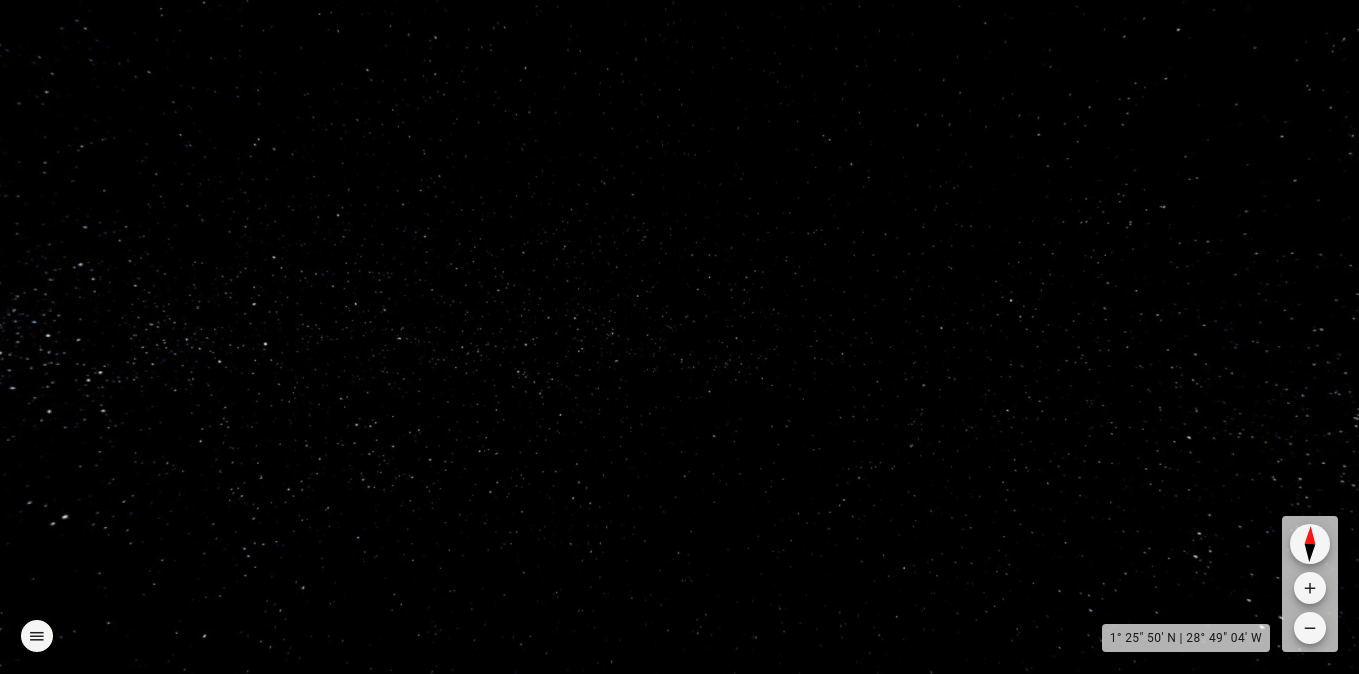
\includegraphics[width=\linewidth]{img/c4_starsVis.png}
    \caption{Wizualizacja gwiazd - klasa \texttt{StarsVis}}
    \label{fig:c4_starsVis} 
\end{figure}

Na listingu~\ref{lst:starsVis} pokazano część klasy \texttt{StarsVis} definiującą tę wizualizację. Kula tworzona jest z użyciem klasy \texttt{THREE.SphereGeometry}, a jej materiał \texttt{THREE.MeshBasicMaterial} zawiera ustawienia definiujące jej wyświetlanie. Ustawienie \mbox{\texttt{side:THREE.BackSide}} sprawia, że teksturowane są odwrotna niż zwykle strona rysowanego trójkąta. Ustawienia \mbox{\texttt{depthWrite:false}} oraz \mbox{\texttt{depthFunc:THREE.NeverDepth}} sprawiają, że obiekt nie będzie wpływał na wartość z-bufora, oraz będzie rysowany zawsze za innymi obiektami, co jest oczekiwane od obiektu tła. 


\begin{lstlisting}[float, language=javascript, label={lst:starsVis}, caption={
    Fragmenty klasy \texttt{StarsVis}}
]
/* ... */
export default class StarsVis extends Visualization {
  private stars = new THREE.SphereGeometry(40000, 10, 10);
  private starsMaterial = new THREE.MeshBasicMaterial({
    side: THREE.BackSide,
    map: new THREE.TextureLoader().load(starsMap),
    depthWrite: false,
    depthFunc: THREE.NeverDepth,
  });
  private mesh = new THREE.Mesh(this.stars, this.starsMaterial);
  /* ... */
  public setupCamera(camera: TrackballCamera): void {
    //
  }
  public setupScene(scene: THREE.Scene, group: THREE.Group): void {
    this.mesh.renderOrder = 0;
    group.add(this.mesh);
  }
  public update(deltaFactor: number): void {
    this.mesh.rotation.y = TimeService.getHourAngle();
  }
  /* ... */
}
\end{lstlisting}

Obiekt 3D \texttt{THREE.Mesh} w metodzie \texttt{update} obracany jest w osi $OY$ o pewien kąt. Kąt ten wynika z czasu słonecznego, ponieważ wizualizacja ta domyślnie ma stanowić tło dla wizualizacji Ziemi w czasie rzeczywistym. Może być ona również rozszerzona, aby obsługiwać każdy inny dowolny czas. Kiedy kamera jest nieruchowa względem punktu na Ziemi, jej obrót w okół własnej osi widoczny jest jako obrót tła w przeciwnym kierunku. Klasa TimeService, dokładniej opisana w dalszej części pracy, zawiera metodę \texttt{getHourAngle}, która dla danej strefy czasowej oblicza kąt obrotu słońca od danej długości geograficznej o danym czasie~\cite{SolarTime}. Punktem odniesienia jest południk $\ang{0}$ i strefa czasowa \textit{+00:00}. 

\section{Atmosfera}